%-------------------------------------------------------------
% $Id$
% © Juan A. de la Puente, 2008
%-------------------------------------------------------------
\documentclass[10pt.a4paper]{memoir}
%\%documentclass[10pt,a4paper]{book}
%-------------------------------------------------------------
\usepackage{natbib}
\usepackage[spanish]{babel}
%% --------- uncomment for use with xetex and mac fonts --------------
%\usepackage[cm-default]{fontspec}
%\usepackage{xunicode}
%\usepackage{xltxtra}
%% -------------------------------------------------------------------------------------
\usepackage[utf8]{inputenc}  % comment if xunicode is used
%% -------------------------------------------------------------------------------------
\usepackage{graphicx}
\usepackage{color}
\usepackage{icomma}
\definecolor{shadecolor}{gray}{0.90}

%% --------- define fonts -----------------------------------------------------------------------
%\defaultfontfeatures{Mapping=tex-text,Scale=MatchLowercase} 
%\setmainfont [Ligatures={Common}, Numbers={OldStyle}]{Garamond}
%%\setmainfont [Ligatures={Common}, Numbers={OldStyle}]{Hoefler Text}
%\setsansfont{Optima Regular} 
%\setmonofont{Monaco} 
%% -------------------------------------------------------------------------------------
%% HEADINGS
%\usepackage{sectsty} 
%\usepackage[normalem]{ulem} 
%\chapterfont{\sffamily}
%\sectionfont{\sffamily\mdseries\large\underline} 
%\subsectionfont{\rmfamily\mdseries\scshape\normalsize} 
%\subsubsectionfont{\rmfamily\bfseries\upshape\normalsize} 
%% -------------------------------------------------------------------------------------
\graphicspath{{figuras/}}

\maxsecnumdepth{chapter} % sólo se numeran los capítulos
\maxtocdepth{section}    % índice hasta secciones

%\newcommand{\ruledsec}[1]{%
%  \noindent\rule{\textwidth}{0.4pt}   \Large\bfseries\raggedright #1 }
%%\noindent\rule{\textwidth}{0.4pt}   \Large\sffamily\raggedright #1 }
%\setsecheadstyle{\ruledsec}
%%\setsubsecheadstyle{\large\itshape\raggedright} 
\setsubsubsecheadstyle{\normalsize\itshape\raggedright}

\newcounter{ejem}[chapter]
\newenvironment{ejemplo}{
\refstepcounter{ejem} 
\begin{framed}\sffamily\noindent\textbf{Ejemplo \thechapter.\theejem.} }
 {\end{framed}}

\makeindex

%-------------------------------------------------------------
\begin{document}
 %-------------------------------------------------------------
\pagestyle{empty}
%-------------------------------------------------------------
% $Id$
% © Juan A. de la Puente, 2008
%-------------------------------------------------------------
% portadilla
\vspace*{\fill}
\begin{center}
\Huge Manual de navegación para yates
\end{center}
\vspace*{\fill}
\cleardoublepage

% portada
\vspace*{\fill}
\begin{center}
\Huge Manual de navegación para yates
\end{center}
\begin{center}
\LARGE\textsf{Juan Antonio de la Puente}\par
\end{center}
\vspace*{\fill}
\clearpage

%página de derechos
\begingroup
\footnotesize
\setlength{\parindent}{0pt}
\setlength{\parskip}{\baselineskip}

\textcopyright{} 2008 Juan Antonio de la Puente Alfaro\\
Reservados todos los derechos

Impreso en España --- Printed in Spain

ISBN

\endgroup
\clearpage
\frontmatter
\pagenumbering{Roman}
%\pagestyle{headings}
\pagestyle{ruled}
\tableofcontents
%\listoffigures
%\listoftables
%-------------------------------------------------------------
\mainmatter
\pagestyle{companion}
%\setsecheadstyle{\Large\itshape\raggedright} 
%\chapterstyle{bianchi}
%\chapterstyle{ger}
%-------------------------------------------------------------
% $Id$
% © Juan A. de la Puente, 2008
%-------------------------------------------------------------
\chapter{Fundamentos de la navegación marítima}
\label{ch:introduccion}
%===================================
\section{La navegación}

\index{navegación|textbf}
\index{pilotaje|textbf}
\index{situación|textbf}
\index{derrota|textbf}

La \emph{navegación} o \emph{pilotaje} tiene por objeto gobernar un barco de forma que llegue a su destino de la forma más segura y rápida posible. Para ello se necesita: 
\begin{itemize}
\item Conocer la \emph{situación} actual del barco;
\item Decidir cuál es la \emph{derrota} (es decir la trayectoria) que hay que seguir para llegar al destino fijado.
\end{itemize}

La navegación es a la vez una técnica y un arte. La técnica de la navegación se apoya en conocimientos  propios de las matemáticas, la física, la astronomía y otras ciencias, con objeto de desarrollar métodos precisos para conocer la situación y determinar la derrota más conveniente. Además de estos métodos, un buen navegante utiliza su experiencia e intuición para valorar la información que obtiene por medio de sus sentidos y de los instrumentos de navegación, evaluar la cercanía y naturaleza de los peligros y, en definitiva, gobernar el barco de la manera más segura y rápida posible. En este manual se describen muchos de los fundamentos científicos y de los métodos que constituyen la técnica de la navegación. El arte de la navegación, sin embargo, sólo se puede aprender navegando, preferentemente en compañía de otros navegantes más expertos. También es útil, aunque de ninguna manera puede sustituir a la experiencia, leer o escuchar relatos de navegación. 

%-------------------------------------------------------------
\subsection{Tipos de navegación}

\index{navegación!costera}
\index{navegación!de altura}

Atendiendo a la zona por donde se navega se pueden distinguir diversos tipos de navegación: 
\begin{itemize}
\item \emph{Navegación costera} es la que se realiza a la vista de la costa. En este tipo de navegación se pueden tomar como referencia los elementos de la costa que son visibles desde la mar, como faros, montañas, edificios y, en general, todos los puntos destacados que nos pueden ayudar a conocer nuestra situación y a evitar los peligros. 
\item  \emph{Navegación de altura} es la que se efectúa en mar abierto, lejos de la costa. En la navegación de altura no se pueden utilizar como referencia puntos situados en tierra, por lo que se hace necesario utilizar técnicas basadas en la observación de los astros o en la recepción de señales radioeléctricas.
\end{itemize}

%-------------------------------------------------------------
\subsection{Técnicas de navegación}

\index{navegación!costera}
\index{navegación!de estima}
\index{navegación!con radar}
\index{navegación!por satélite}
\index{navegación!astronómica}

El navegante tiene a su disposición diversas técnicas para obtener su situación y elegir el rumbo que ha de seguir en cada momento. Algunas de estas técnicas son muy antiguas, como las basadas en la enfilación de marcas en tierra, cuyo origen es anterior a la historia escrita. Otras datan sólo de hace unos pocos años, como la navegación por satélite. Las técnicas de navegación que actualmente se pueden considerar más útiles para un yate de tamaño medio se pueden agrupar en las siguientes categorías: 
\begin{itemize}
\item \emph{Navegación costera}: esta categoría comprende un conjunto de técnicas basadas en la observación de puntos situados en tierra, como son las basadas en enfilaciones, demoras, distancias y ángulos horizontales. 
\item \emph{Navegación de estima}: se basa en el cálculo aproximado de la derrota seguida a partir del rumbo y de la distancia navegada. La estima proporciona una situación aproximada, que resulta útil como comprobación de la obtenida por otros métodos más exactos, o cuando no se pueden emplear éstos por algún motivo. 
\item \emph{Navegación con radar}: se basa en el uso del radar para determinar la dirección y la distancia a la que se encuentra la costa y otros obstáculos a la navegación, como pueden ser las rocas aisladas o los barcos próximos. 
\item \emph{Navegación por satélite}: se basa en la recepción de señales de radio emitidas por satélites artificiales. Proporciona una situación muy precisa. 
\item \emph{Navegación astronómica}: se basa en la observación de la posición de los astros ---el Sol, la Luna, los planetas o algunas estrellas--- en el firmamento. Proporciona situaciones bastante precisas, aunque no tanto como la navegación por satélite. 
\end{itemize}

Ninguna técnica de navegación es suficiente por sí sola, por lo que un buen navegante debe conocer todos los métodos que pueden resultarle útiles teniendo en cuenta el tamaño de su barco y el tipo de navegación que quiera realizar. En particular, no debe confiarse sólo en la navegación por satélite, aunque actualmente sea la más fácil de llevar a cabo y 
la que proporciona situaciones más precisas. La dependencia de sistemas basados en satélites, cuyo funcionamiento puede verse alterado de forma imprevisible, y la posibilidad de averías en los receptores que se utilizan (como en cualquier instrumento de navegación) aconsejan el uso simultáneo de otros métodos. 

%===================================
\section{La Tierra}

\index{Tierra|textbf}
\index{Tierra!forma|see{geoide, elipsoide}}
\index{Tierra!polos|see{polos}}
\index{Tierra!ecuador|see{ecuador}}
\index{Tierra!paralelos|see{paralelo}}
\index{Tierra!meridianos|see{meridiano}}

\index{polos|textbf}
\index{polos!polo Norte}
\index{polos!polo Sur}
\index{ecuador|textbf}
\index{paralelo|textbf}
\index{meridiano|textbf}
\index{meridiano!inferior}

\index{Norte}
\index{Sur}

La navegación se efectúa sobre la superficie del mar, que constituye la mayor parte de la superficie terrestre. La forma de la Tierra, como es sabido, se aproxima a la de una esfera achatada en los polos. En la mayoría de los casos no se comete error apreciable si se supone que su forma es completamente esférica, por lo que así lo haremos, excepto cuando sea necesario. 

La Tierra gira sobre sí misma alrededor de un eje, cuyos extremos se denominan \emph{polo Norte} y \emph{polo Sur}. El círculo máximo perpendicular al eje terrestre se llama \emph{ecuador}, y los círculos menores paralelos al mismo se denominan \emph{paralelos}. Los \emph{meridianos} son círculos máximos que pasan por los polos. Se denomina \emph{meridiano de un lugar } al semicírculo que va de un polo al otro pasando por el lugar. El \emph{meridiano inferior} de un lugar es el otro semicírculo del mismo meridiano, es decir es el meridiano que se sitúa en los antípodas (figura~\ref{fg:esfera}).

\begin{figure}[hbtp]
\begin{center}
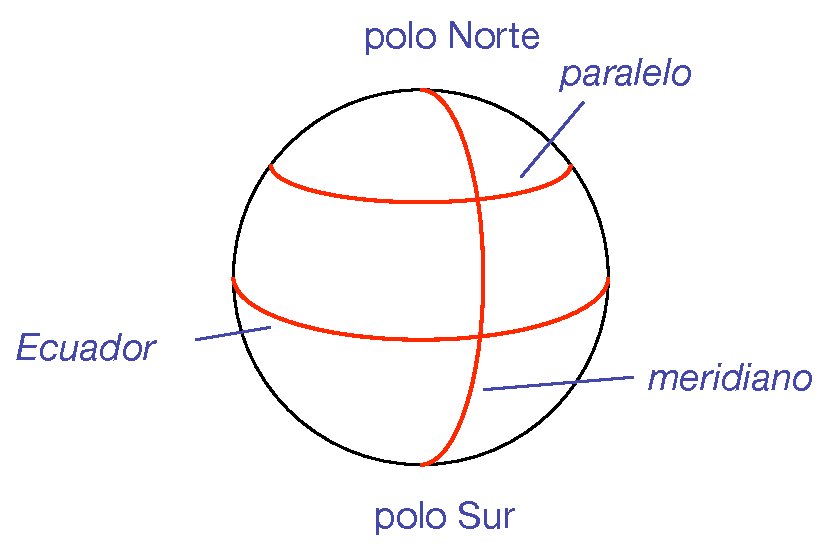
\includegraphics[scale=0.45]{esfera}\\
\caption{Esfera terrestre}
\label{fg:esfera}
\end{center}
\end{figure}


%-------------------------------------------------------------
\subsection{Coordenadas geográficas}

\index{coordenadas|textbf}
\index{coordenadas!geográficas}
\index{coordenadas!latitud|textbf}
\index{coordenadas!longitud|textbf}

%···················································································
\subsubsection{Latitud y longitud}

\index{latitud|textbf}
\index{longitud|textbf}
\index{meridiano!de referencia|textbf}
 \index{meridiano!primer \textemdash|see{meridiano de referencia}}
 \index{meridiano!origen|see{meridiano de referencia}}
 \index{meridiano!de Greenwich} 
 
 \index{Norte}
 \index{Sur}
 \index{Este}
 \index{Oeste}
 
Para situar un punto cualquiera en la superficie de la Tierra se utilizan sus dos \emph{coordenadas geográficas} (figura \ref{fg:coordenadas}): 
\begin{itemize}
\item La \emph{latitud} es el arco de meridiano comprendido entre el ecuador y el punto. Se mide en grados y minutos%
\footnote{Un grado se divide en sesenta minutos, y un minuto en sesenta segundos. Actualmente se prefiere usar fracciones decimales de minuto en vez de segundos. Por ejemplo, 38º 37’ 42” =  38º 37,7’. }
hacia el Norte o hacia el Sur, y su valor está comprendido entre 0º y 90º. 
\item La \emph{longitud} de un punto es el arco de ecuador comprendido entre un \emph{meridiano de 
referencia} o \emph{primer meridiano} y el meridiano que pasa por el punto. Se mide igualmente en grados y minutos, hacia el Este o hacia el Oeste, y su valor está comprendido entre 0º y 180º. Al no haber ningún meridiano que se presente de forma natural como origen para la medida de la longitud, se adopta como meridiano de referencia uno cualquiera, atendiendo a razones de conveniencia. Por convenio internacional el primer meridiano es el \emph{meridiano de Greenwich}, que pasa por el observatorio situado en la ciudad inglesa de ese mismo nombre.%
\footnote{Antiguamente cada país usaba un meridiano de referencia propio. En España se han utilizado como tales los de  la isla del Hierro (punta Orchilla), San Fernando o Cádiz y Madrid, entre otros.} %
\end{itemize}

\begin{figure}[hbtp]
\begin{center}
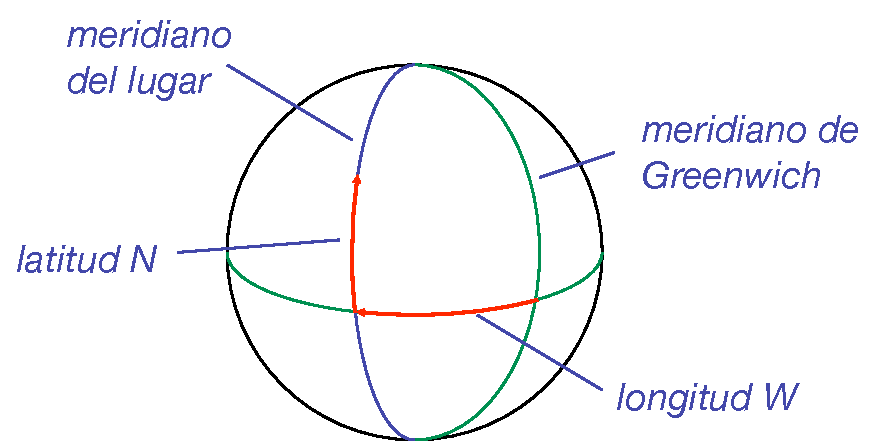
\includegraphics[scale=0.45]{coordenadas}\\
\caption{Coordenadas geográficas}
\label{fg:coordenadas}
\end{center}
\end{figure}

Generalmente se usan las abreviaturas $l$ y $L$, respectivamente, para la latitud y la longitud,%
\footnote{También se usan los símbolos $\phi$ y $\lambda$, respectivamente, para la latitud y la longitud.} 
 y N, S, E y W para las direcciones de los puntos cardinales Norte, Sur, Este y Oeste. La situación de un punto se indica mediante su latitud y longitud, en este orden. Los minutos se escriben generalmente con dos cifras. Normalmente se dan las coordenadas con décimas de minuto, siempre que la situación haya sido obtenida con suficiente precisión. 
 
 \begin{ejemplo}
La latitud del faro del Estacio es \mbox{37º 44,5’ N}, y su longitud \mbox{0º 43,4’ W}. 
Por tanto, su situación es \mbox{37º 44,5’ N 0º 43,4’ W.} 
\end{ejemplo}

%···················································································
\subsubsection{Diferencias de latitud y longitud}

\index{latitud!diferencia}
\index{longitud!diferencia}
 
La \emph{diferencia de latitud} $\Delta l$ entre dos puntos es la resta algebraica de sus latitudes, considerando las latitudes Norte como positivas y las latitudes Sur como negativas. La \emph{diferencia de longitud} $\Delta L$ entre dos puntos es la resta algebraica de sus longitudes, considerando las longitudes Este como positivas y las longitudes Oeste como negativas.%
\footnote{Seguimos aquí el convenio de la Unión Astronómica Internacional (UAI). En algunos manuales de navegación se sigue el convenio contrario, es decir se consideran positivas las longitudes Oeste. El convenio de signos de la UAI tiene ventajas en los cálculos de horas y de estima analítica (ver capítulo \ref{ch:estima}).}

\begin{ejemplo}
La diferencia de latitud y longitud entre el faro del Estacio  y el bajo de En Pou, en el freu grande de Ibiza, situado en
\mbox{38º 48,3' N 1º 25,1' E},  es: 

\[
\begin{array}{lll}
\mbox{Bajo de En Pou}       & +38º \, 48,3’ \:  \mathrm{N}   &   +1º \, 25,1’ \: \mathrm{E}  \\
\mbox{Faro del Estacio}      & +37º \, 44,5’  \: \mathrm{N}   &   -0º  \,43,4’   \:  \mathrm{W}  \\
\hline
 \mbox{Diferencia}               & + \;\;1º  \, 03,8’ \: \mathrm{N}   &    +2º \, 08,5’  \: \mathrm{E} 
\end{array}
\]

Por tanto, el bajo d’En Pou está 1º 03,8’ al Norte y 2º 08,5’ al Este del faro del Estacio. 
\end{ejemplo}

%-------------------------------------------------------------
\subsection{Dirección y distancia }

%···················································································
\subsubsection{Medida de direcciones}

\index{dirección}
\index{rumbo|textbf}
\index{línea!loxodrómica|textbf}

Los marinos miden la dirección de una línea por medio del ángulo que forma con una dirección de referencia. Algunos de estos ángulos tienen un nombre específico. En particular, el ángulo que forma la dirección que sigue un barco con la dirección Norte se llama \emph{rumbo}.  Los rumbos se miden de 0º a 360º a partir del Norte,  en el sentido de las agujas del reloj (figura \ref{fg:rumbo}).

\begin{figure}[hbtp]
\begin{center}
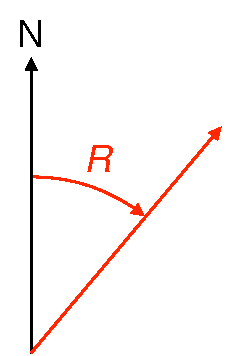
\includegraphics[scale=0.45]{rumbo}\\
\caption{Rumbo}
\label{fg:rumbo}
\end{center}
\end{figure}

Las líneas que forman un ángulo constante con los meridianos (es decir con el Norte) se llaman \emph{líneas loxodrómicas}. Los barcos suelen seguir líneas loxodrómicas en su navegación, ya que para ello basta con mantener un rumbo constante.

%···················································································
\subsubsection{Medida de distancias}

\index{distancia}
\index{distancia!ortodrómica|textbf}
\index{distancia!loxodrómica!textbf}
\index{milla náutica|textbf}
\index{cable|textbf}
 
La unidad de distancia que se usa en navegación es la \emph{milla náutica }($M$),%
\footnote{No existe un acuerdo general sobre el símbolo que se debe usar para la milla náutica. El símbolo $M$ es el recomendado por la Oficina Internacional de Pesos y Medidas.}
 que mide 1852~m, valor aproximadamente igual a la longitud media de 1 minuto de arco de meridiano.%
\footnote{El aplanamiento de la Tierra hace que la longitud de 1' de meridiano varíe ligeramente con la latitud, de manera que su valor es de unos 1843~m en el ecuador, y unos 1861~m en los polos.}

La distancia más corta entre dos puntos situados en una superficie esférica es igual a la longitud del arco de círculo máximo que los une. Su valor se llama \emph{distancia ortodrómica}. Sin embargo, en muchos casos la distancia se mide sobre la línea loxodrómica que une los dos puntos. En este caso se habla de\emph{ distancia loxodrómica}, o \emph{distancia} a secas. En distancias cortas (de menos de 500 millas) no hay error apreciable al medir la distancia loxodrómica en vez de la ortodrómica. 

\begin{ejemplo}
La distancia (ortodrómica) entre el puerto Tomás Maestre, en La Manga, y el Freu Grande de Ibiza es de 119,8~M.. La distancia loxodrómica  entre estos dos puntos es de 120,2~M. Como puede verse, la diferencia no es significativa para distancias de este orden. 

Por otra parte, la distancia ortodrómica entre Vigo y  Nueva York es de 2861~M, mientras que la distancia loxodrómica correspondiente es de 2945~M. Para grandes distancias, por tanto, la diferencia es importante.
\end{ejemplo}

Las distancias menores que una milla se miden en metros, aunque en ocasiones todavía se usa como unidad de medida el \emph{cable}, que equivale a la décima parte de una milla, es decir 185,2~m.

%-------------------------------------------------------------
\subsection{Elipsoide de referencia y datum}

\index{geoide|textbf}
\index{elipsoide|textbf}
\index{elipsoide!de referencia}
\index{datum}
\index{datum!europeo (Potsdam)}
\index{datum!horizontal|textbf}

\index{sistema geodésico mundial|see{WGS84}}
\index{World Geodetic System|see{WGS84}}
\index{WGS,WGS84|textbf}
 
El hecho de que la Tierra no sea perfectamente esférica afecta a la forma de medir la latitud y la longitud. La forma real de la Tierra, suponiendo que toda su superficie estuviera ocupada por los océanos, es una figura geométrica irregular denominada \emph{geoide}. Para calcular las coordenadas geográficas de un punto se aproxima el geoide por un \emph{elipsoide de revolución}, figura que se obtiene al hacer girar una elipse sobre uno de sus ejes (en este 
caso el eje menor). Al ser el geoide irregular, el elipsoide que mejor se ajusta a la forma de la Tierra es diferente para cada zona de la Tierra, y ello ha dado lugar a la utilización de distintos \emph{elipsoides de referencia} por los servicios cartográficos e hidrográficos de los distintos países. Se denomina \emph{datum horizontal} al conjunto de parámetros que se utilizan para determinar las coordenadas geográficas en una zona determinada, a partir de un elipsoide de referencia. 

En Europa se solía usar hasta hace pocos años el llamado \emph{datum europeo}, basado en un elipsoide internacional que se ajusta con el geoide en Potsdam (Alemania). En otros continentes se usan otros datos, como el datum de Norteamérica, el de la India o el de Tokio. Todos ellos han sido sustituidos por el \emph{ sistema geodésico internacional} (\emph{world geodetic system}), más conocido por las siglas WGS84. Este sistema de referencia está ajustado de forma que permite calcular las coordenadas geográficas de puntos situados en cualquier lugar del globo con un error mínimo. 
Las diferencias entre las coordenadas calculadas con respecto a uno u otro datum son pequeñas, generalmente inferiores a 0,1’. Estas diferencias no son significativas cuando se usan métodos poco precisos para calcular la situación de un punto, pero cuando se usan métodos de navegación basados en satélites, que permiten determinar la situación con una precisión de algunos metros, es necesario tenerlas en cuenta. Las cartas españolas, cuando están basadas en el datum europeo,  suelen indicar la diferencia entre las situaciones marcadas en la carta y las referidas al sistema WGS84 (véanse los capítulos \ref{ch:cartas} y \ref{ch:gps}). 

%-------------------------------------------------------------
\subsection{El campo magnético terrestre}
 
\index{Tierra!campo magnético|textbf}
\index{polos!magnéticos}
\index{polos!polo Norte!magnético}
\index{polos!polo Sur!magnético}

\index{declinación|textbf}
\index{declinación!magnética}
\index{declinación!incremento anuo}
\index{declinación!decremento anuo}
\index{variación magnética|see{declinación}}

\index{Norte}
\index{Norte!geográfico}
\index{Norte!verdadero|textbf}
\index{Norte!magnético|textbf}

\index{meridiano|textbf}
\index{meridiano!inferior}
 
La Tierra tiene un campo magnético de intensidad apreciable, orientado aproximadamente en dirección Norte-Sur. Se llama \emph{Norte magnético} a la dirección hacia la que se orienta espontáneamente un imán o una aguja imantada (es decir, una brújula) por efecto del campo magnético terrestre.

El ángulo que forma el Norte magnético con el Norte geográfico o \emph{Norte verdadero} se llama \emph{declinación} o \emph{variación magnética} (figura \ref{fg:declinacion}). Su valor se mide en grados, y es positivo (NE) cuando el Norte magnético está hacia el Este del Norte verdadero, y negativo (NW) cuando el Norte magnético está al Oeste del verdadero. El valor de la declinación se suele representar mediante el símbolo $d_{m}$ o $\delta$. 

La declinación magnética, y por tanto la dirección del Norte magnético, varía para cada lugar de la Tierra. Además, su valor cambia con el tiempo, llamándose \emph{incremento} o \emph{decremento anuo} la diferencia de valor de la declinación entre un año y el siguiente. Las cartas y otros documentos náuticos (ver capítulo \ref{ch:cartas}) proporcionan el valor de la declinación y su diferencia anua en las zonas que cubren. 

\begin{ejemplo}
La declinación magnética en las cercanías del cabo de la Nao en 2004 era de 1º W, con una diferencia anual de 7’ E. En este caso la declinación es negativa y la diferencia es positiva. Si queremos calcular el valor de la declinación en 2009 efectuaremos las siguientes operaciones: 
\[ 
\begin{array}{lcll}
\mbox{Valor en 2004 } &   = &  -1º \, 00’ \: \mathrm{(W) } \\
\mbox{Diferencia}         &   = &   +0º \, 35’ \: \mathrm{(E)}  &(\mbox{5 años} \times 7' )\\
\mbox{Valor en 2009}  &  = &   -0º \, 25’ \: \mathrm{(W)} & \approx -0,5º 
\end{array}
\]
\end{ejemplo}

El valor de la declinación se suele dar en grados y minutos enteros o en grados y décimas de grado. 

%===================================
\section{El tiempo}

\index{tiempo|textbf}
\index{segundo|textbf}
\index{sistema internacional de unidades}
\index{SI|see{sistema internacional de unidades}}

 
La medida precisa del tiempo es de gran importancia para la navegación. El tiempo transcurrido desde la última situación nos permite calcular la distancia recorrida, si conocemos la velocidad del barco. La determinación exacta del instante de las observaciones es fundamental en navegación astronómica, y la navegación por satélite hace uso de relojes atómicos de gran precisión para medir el tiempo que tardan las señales radiadas en llegar al observador. Por tanto, el navegante debe ser capaz de conocer la hora en todo momento con la precisión necesaria para el tipo de navegación que esté efectuando. 

Desde la antigüedad más remota se ha medido el tiempo a partir de la observación de los fenómenos astronómicos más evidentes: la rotación de la Tierra, a partir de la cual se define la duración del día y su división en horas, minutos y segundos, y su traslación alrededor del Sol, cuya duración es de un año. La observación de las fases de la Luna dio origen, por su parte, a la semana y el mes. 

A medida que se dispuso de relojes e instrumentos astronómicos más precisos se observó, sin embargo, que estos fenómenos astronómicos presentan irregularidades. Ello dio lugar a definiciones más precisas de las unidades de tiempo, hasta llegar a la época actual, en que la medida del tiempo se basa en la observación de fenómenos atómicos de 
una gran regularidad. Actualmente todas las medidas de tiempo se refieren al Sistema Internacional de unidades (SI),  cuya unidad fundamental es el \emph{segundo} ($s$). Esta unidad se define a partir de la frecuencia de la radiación emitida por un átomo de Cesio.%
\footnote{La duración del segundo se define como $9\,192\,631\,770$ períodos de la radiación correspondiente a la transición entre los dos niveles hiperfinos del átomo de Cs\textsuperscript{133}. }
Para los usos prácticos, sin embargo, se mantienen las unidades de tiempo tradicionales, estableciéndose formalmente su relación con la unidad fundamental: 

\begin{tabular}{lcl}
1 minuto &= &60 segundos\\
1 hora     &= &60 minutos\\
\end{tabular}

Normalmente se da la hora del día en horas y minutos, o en horas, minutos y segundos. Se suelen dar los valores respectivos separados por sus abreviaturas (h, m, s) o por el signo “:” (dos puntos). Cuando se dan sólo las horas y minutos se pueden escribir con las cuatro cifras respectivas sin separación. 

\begin{ejemplo}
Las siguientes expresiones se refieren a la misma hora: 

\begin{center}
\begin{tabular}{lll}
3h 45m & 03:45 & 0345 \\
\end{tabular}
\end{center}
\end{ejemplo}

\index{sistema de referencia de tiempo}
\index{sistema de referencia de tiempo!\textemdash|seealso{tiempo solar, tiempo solar medio, tiempo universal}}

La expresión de la hora del día está sujeta a un \emph{sistema de referencia de tiempo}. A continuación se describen de forma resumida los sistemas de referencia más usados en navegación. 

%-------------------------------------------------------------
\subsection{Tiempo solar}

\index{tiempo!solar}
\index{día!solar}

El tiempo solar se mide a partir del movimiento aparente del Sol. Un \emph{día solar} es el tiempo que transcurre entre dos pasos sucesivos del Sol por el meridiano de un lugar. El día solar se divide en 24 \emph{horas solares}, y la \emph{hora solar} es el número de horas solares transcurridas desde el paso del Sol por el meridiano inferior del lugar. 

El tiempo solar no se utiliza apenas, ya que la forma elíptica de la órbita de la Tierra en torno al Sol, la inclinación del eje de la Tierra sobre el plano de esa misma órbita (denominado \emph{plano de la eclíptica}), y algunas otras irregularidades hacen que la duración del día solar presente notables variaciones a lo largo del año.%
\footnote{La diferencia entre el día solar más corto y el más largo es de algo más de 30~minutos.}

%-------------------------------------------------------------
\subsection{Tiempo solar medio}

\index{tiempo!solar medio}
\index{día!solar medio}
\index{hora!solar media}
\index{hora!civil}

Para evitar las irregularidades del tiempo solar se utiliza el \emph{tiempo solar medio}, basado en la duración media del día solar y en la aproximación del movimiento real de la Tierra por otro imaginario en el que se considera que la órbita de la Tierra es circular y su eje es perpendicular al plano de la eclíptica. El movimiento aparente del Sol en esta aproximación se denomina \emph{Sol medio}, y es regular a lo largo del año. De esta manera se define el \emph{día 
solar medio} como la duración media del día solar. El día solar medio tiene una duración aproximadamente igual a 24 horas. La \emph{hora solar media} u \emph{hora civil} de un lugar es el tiempo transcurrido desde el paso del Sol medio por el meridiano inferior del lugar, o lo que es lo mismo desde la medianoche del día solar medio. 

%-------------------------------------------------------------
\subsection{Tiempo universal}

\index{tiempo!universal}
\index{hora!universal|seealso{tiempo universal}}
\index{hora!civil!de Greenwich|seealso{tiempo universal}}
\index{TU|see{tiempo universal}}
\index{UT|see{tiempo universal}}

Como el Sol pasa en distintos momentos por el meridiano de cada lugar, la hora civil será diferente para cada lugar de la Tierra, aunque todos los lugares situados en el mismo meridiano tienen la misma hora civil. Para evitar los inconvenientes que ello acarrea conviene definir un \emph{tiempo universal} que sirva de referencia para toda la Tierra. Por convenio internacional se toma como tiempo universal el tiempo solar medio del meridiano de Greenwich, u \emph{hora civil de Greenwich}. Para designar el tiempo universal se usan las abreviaturas TU o UT (\emph{universal time}).%
\footnote{Está en desuso la abreviatura GMT (\emph{Greenwich Mean Time}) que se usaba para designar el tiempo universal.}

%...................................................................................
\subsubsection{Hora civil y hora universal}

\index{hora!civil}
\index{hora!universal}

La hora civil de los lugares que están situados en meridianos diferentes del de Greenwich está relacionada con la hora universal por la longitud. Como el día solar medio dura 24~horas, y esto equivale a una rotación de 360º, la Tierra gira 15º ($= 360/24$) cada hora. En consecuencia, los lugares que están 15º al Oeste del meridiano de Greenwich tienen 
una hora civil que es una hora anterior a la hora universal, y así sucesivamente. En general, la fórmula que relaciona la hora civil de un lugar (HcL) con la hora universal (TU) es: 
\begin{equation}
\mathrm{HcL} = \mathrm{TU} + \Lambda
\end{equation}
donde $\Lambda$ es el equivalente en tiempo de la longitud, 
\begin{equation}
\Lambda = \frac{L}{15}
\end{equation}
$L$ se expresa en grados y fracciones de grado. Hay que tener en cuenta el convenio de signos para la longitud (positiva al Este) para aplicar esta fórmula. 

\begin{ejemplo}
La hora civil en Cedeira (43º 39,7’ N 8º 3,2’ W) cuando son las 15h 37m TU es 
\[
\begin{array}{lcrr}
  \mathrm{TU} &  =  &   23 & 58 \\
  \Lambda        &  =  &   -00 & 32\\ \cline{3-4}
  \mathrm{HcL} &   = &   15 &05\\
\end{array}
\]
El valor de $\Lambda$ se calcula dividiendo 8,05 ($\mathsf{= 8+3.2/60}$) por 15. El resultado es $0.54$ horas, es decir 32 minutos ($\mathsf{=0.54 \cdot 60}$). El valor es negativo por ser la longitud Oeste. 
\end{ejemplo}

Hay que tener en cuenta que la hora civil en un lugar determinado puede corresponder a una fecha distinta de la correspondiente a la hora universal. 

\begin{ejemplo}
La hora civil en Mahón (39º 52,1’ N 4º 18,6’ E) cuando son las 23h 58m TU del día 8 de abril es: 
\[
\begin{array}{lcrrl}
  \mathrm{TU} &  =  &   23 & 58 \\
  \Lambda        &  =  &   +00 & 17\\ \cline{3-4}
  \mathrm{HcL} &   = &   00 & 15 & \mbox{(día 9 de abril)}\\
\end{array}
\]
es decir, las 00h 15m del día siguiente. 
\end{ejemplo}

%-------------------------------------------------------------
\subsection{Tiempo universal coordinado}

\index{tiempo!universal coordinado|textbf}
\index{UTC|see{tiempo universal coordinado}}
\index{TUC|see{tiempo universal coordinado}}
\index{hora!universal}
\index{hora!UTC}

El tiempo universal coordinado (TUC o UTC, \emph{Universal Time Co-ordinated}) se basa en el empleo de relojes atómicos, ajustados de tal manera que su valor no difiera en más de 0,9~s del tiempo universal basado en observaciones astronómicas. El TUC es la base de la hora oficial en todos los países del mundo. 

En lo sucesivo consideraremos que el TU y el TUC son equivalentes. 

%-------------------------------------------------------------
\subsection{Hora legal}

\index{hora!legal}
\index{huso horario|textbf}
\index{zona horaria}
\index{zona horaria!\textemdash|seealso{huso horario}}

El hecho de que la hora civil de lugares próximos sea diferente hace su uso poco práctico para la vida diaria. Para evitar este inconveniente se suele adoptar una misma \emph{hora legal} para una zona de la Tierra. Con este fin se divide la superficie terrestre en 24 \emph{husos horarios} de 15º de longitud cada uno, centrados en los meridianos 0º, 15º, etc. (figura \ref{fg:husos}). 

\begin{figure}[hbtp]
\begin{center}
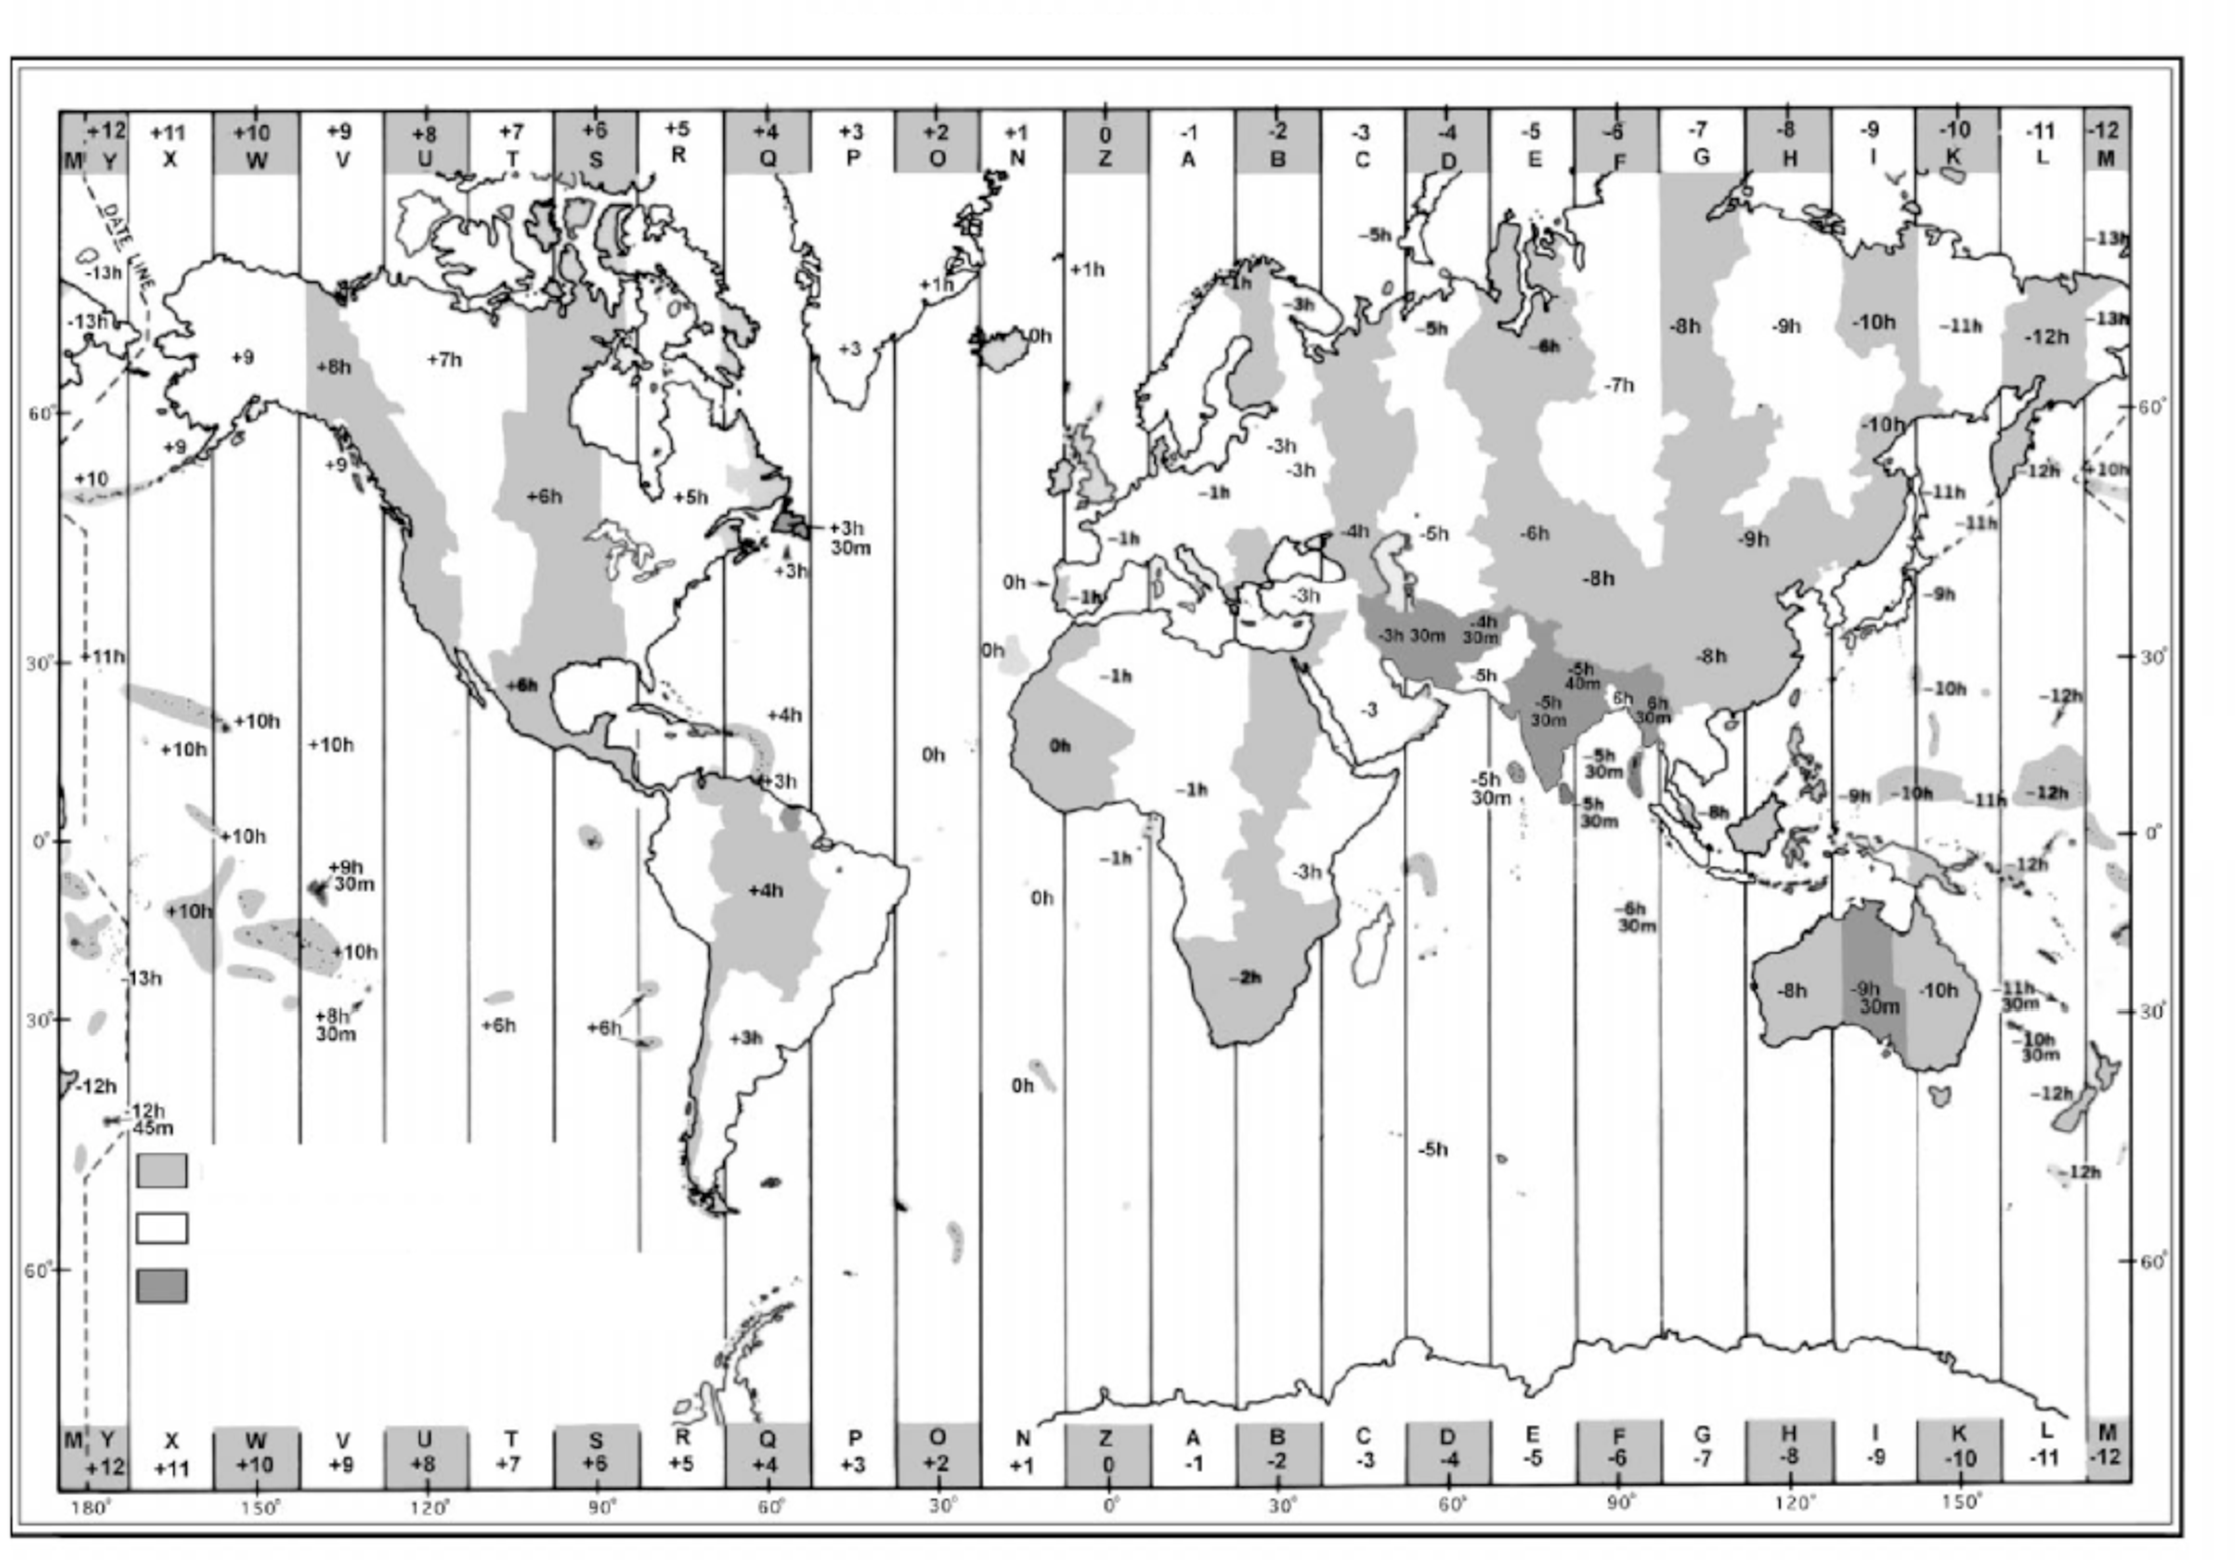
\includegraphics[width=\textwidth]{husos}\\
\caption{Husos horarios y zonas de hora legal}
\label{fg:husos}
\end{center}
\end{figure}

Todos los lugares que están en un mismo huso horario tienen la misma hora legal. En algunas partes del mundo se usan zonas horarias que no coinciden exactamente con los husos horarios. Por ejemplo, toda la parte peninsular de España está incluida en la zona 0, aunque estrictamente hablando la parte occidental de Galicia pertenece al huso -1. Las Islas Canarias se encuentran en su totalidad en la zona -1. 

La hora legal (Hl) de un lugar está relacionada con la hora universal por la ecuación: 
\begin{equation}
\textrm{Hl} = \mathrm{TU} + Z
\end{equation}
donde $Z$ es la zona o huso horario en que se encuentra el lugar. 

En alta mar el valor de Z es 
\begin{equation}
Z = \mathrm{entero}\left(\frac{L}{15}\right)
\end{equation}
pero en puerto y en aguas territoriales la hora legal será la que corresponda a la zona horaria del lugar en que nos encontremos.

La función \textit{entero} da el valor entero redondeado más próximo a su argumento.  Por ejemplo, 
$\mathrm{entero}(1,2) = 1$, pero $\mathrm{entero}(1,7) = 2$.

\begin{ejemplo}
Se desea obtener la hora legal en un lugar situado en \mbox{40º 35,0’\:N} 37º 12,7’ W cuando son las 0235 TU.

En primer lugar se calcula la zona horaria:
\[ Z  = \mathrm{entero}(-37.21/15)  =  \mathrm{entero}(-2.48) =  -2 \]
teniendo en cuenta que $ 37º 12.7’ = 37+12.7/60 = 37.21º $.

 La hora legal se calcula de la siguiente forma:
\[
\begin{array}{lcrr}
  \mathrm{TU} & =  &  02 & 35 \\
  Z                     & = &   -02 &00 \\ \cline{3-4}
  Hl                    & = & 00 & 35
\end{array} 
\]

\end{ejemplo}

%...................................................................................
\subsubsection{Línea de cambio de fecha}

\index{línea!de cambio de fecha}

El meridiano 180º puede considerarse indistintamente Este u Oeste. Por tanto, se puede considerar que la hora en el mismo es 12 horas anterior o 12 horas posterior al TU. Para resolver esta ambigüedad se conviene en cambiar la fecha al llegar a dicho meridiano, de forma que cuando se va hacia el Este se cuenta un día menos y cuando se va hacia el Oeste 
se cuenta un día más. 

Para evitar los problemas que surgen en las escasas tierras que se encuentran sobre este meridiano, se definió una línea internacional de cambio de fecha que se aparta ligeramente del meridiano 180º en las zonas de tierra (figura \ref{fg:husos}). 

\begin{ejemplo}
Cuando son las 15\,30 TU del día 8 de abril, en el meridiano 175º E son las 03\,30 del
día 9, mientras que en el meridiano 175º W son las 03\,30 del día 8. 
\end{ejemplo}

%-------------------------------------------------------------
\subsection{Hora oficial}

\index{hora!oficial\textbf}
\index{hora!de Europa central (CET)}
\index{horario!de verano}
\index{horario!de invierno}
\index{CET}

En algunos países se modifica la hora legal por motivos políticos o económicos, durante todo el año o durante algunos meses. La \emph{hora oficial} en estos países es igual a la hora legal corregida con un adelanto o retraso: 
\begin{equation}
\mathrm{Ho} = \mathrm{Hl} + C
\end{equation}
donde $C$ es la corrección oficial (adelanto o retraso). En España $C$ es igual a 1~hora en invierno
 y 2horas en verano.%
\footnote{La hora oficial en la España peninsular es la denominada CET (\emph{Central Europe Time}), que es oficial también en la mayoría de los países de Europa Occidental. El horario de verano comienza el último domingo de marzo a las 0100 TU, y termina el último domingo de octubre a la misma hora (0100 TU). En Canarias la correción es la misma, y el cambio de hora se efectúa al mismo tiempo que en la península. Como las islas Canarias están en el huso -1, la hora oficial en Canarias es siempre una hora menos que en la Península.}

%-------------------------------------------------------------
\subsection{El reloj de bitácora}

\index{reloj de bitácora}
\index{hora!del reloj de bitácora (HRB)}
\index{HRB}

El \emph{reloj de bitácora} es el que se usa a bordo de un barco para marcar la hora. Se suele poner en hora con la hora oficial cuando se navega cerca de la costa, o con la hora legal cuando se navega en alta mar. La expresión \emph{hora del reloj de bitácora} (HRB) se refiera a la hora que marca el reloj de bitácora, y es por tanto equivalente a hora oficial u hora legal, según los casos. 

%-------------------------------------------------------------
\subsection{La fecha y el calendario}

\index{fecha}
\index{calendario}

La determinación de la fecha se basa, como es sabido, en el movimiento de traslación de la Tierra alrededor del Sol, cuyo período, denominado \emph{año trópico}, tiene una duración de 365,2425 días aproximadamente. Para ajustar la duración del año a un número entero de días completos se usan las reglas del \emph{calendario gregoriano}, por las cuales se añade un día (el 29 de febrero) a determinados años, denominados \emph{años bisiestos}. Son bisiestos los años cuyo número es múltiplo de 4, excepto los múltiplos de 100 que no lo son de 400 (por ejemplo, el año 2000 fue bisiesto, pero no lo fueron los años 1700, 1800 ni~1900).

%-------------------------------------------------------------
% $Id$
% © Juan A. de la Puente, 2008
%-------------------------------------------------------------
\chapter{Cartas náuticas}
\label{ch:cartas}
%===================================
\section{Cartas náuticas }

\index{cartas náuticas|textbf}

\index{carta|textbf}
\index{carta!náutica}
\index{carta!electrónica}
\index{visor}
\index{plotter|textbf}
\index{avisos a los navegantes}
\index{Instituto Hidrográfico de la Marina|textbf}

Una carta náutica es un mapa de una zona de la superficie del mar y de la costa adyacente.
Las cartas muestran la forma de la costa, la profundidad del mar, los puntos peligrosos para 
la navegación, las ayudas a la navegación, los puntos relevantes de la costa, y todos los 
detalles útiles para navegar en la zona que cubren. 

Las cartas pueden presentarse de distintas formas. La más común es la carta impresa 
sobre una superficie de papel, pero cada vez son más frecuentes las \emph{cartas electrónicas}, 
cuyo contenido está codificado en forma numérica y almacenado en un dispositivo electrónico adecuado. Las cartas electrónicas no son simplemente una versión digital de las cartas 
en papel, sino que pueden contener información adicional, que se puede consultar de distintas formas, y mezclar con los datos obtenidos de otros instrumentos electrónicos. Para 
leer las cartas electrónicas se necesita un visor adecuado, que puede ser un computador 
ordinario dotado de los programas necesarios. Sin embargo es muy frecuente que las cartas electrónicas 
se utilicen con un computador especializado (\emph{plotter}) integrado con otros instrumentos electrónicos, como 
navegadores por satélite o sistemas de radar. 

Los servicios hidrográficos de cada país realizan los trabajos necesarios para recopilar 
los datos necesarios para confeccionar cartas de las zonas de navegación que les interesan, 
y publican cartas oficiales basadas en esos datos y en los que intercambian con otros países. Estos mismos servicios o, en ocasiones, editoriales privadas publican también cartas 
especialmente adaptadas a la navegación deportiva. Es muy importante mantener las cartas 
al día, aplicándoles las correcciones que se publican en los avisos a los navegantes o en 
otras publicaciones similares. En España el Instituto Hidrográfico de la Marina es el organismo encargado de publicar las cartas náuticas oficiales y otros documentos destinados a los navegantes.

%------------------------------------------------------------


\subsection{La proyección de Mercator}

\index{proyección|textbf}
\index{proyección!de Mercator|textbf}
\index{proyección!equivalente}
\index{proyección!isogónica}
\index{proyección!conforme}
\index{línea!ortodrómica}
\index{línea!loxodrómica}
\index{carta!mercatoriana|textbf}



La representación de la superficie de la Tierra, aproximadamente esférica, sobre una superficie plana se realiza mediante una \emph{proyección}. Una proyección es una relación que hace 
corresponder a cada punto de la superficie terrestre un punto del plano de la carta.%
\footnote{En términos matemáticos este tipo de relación se llama \emph{aplicación}. Para construir un mapa de 
forma correcta la aplicación debe ser \emph{biyectiva}, es decir a cada punto de la parte de la superficie terrestre considerada debe corresponder un único punto en la carta y viceversa.}
 Generalmente se procura que la proyección utilizada tenga determinadas características, como la 
conservación de las formas de los accidentes geográficos (proyecciones conformes), de las superficies de los mares y continentes (proyecciones equivalentes), etc. Ninguna proyección 
permite mantener todas estas propiedades a la vez, por lo que generalmente es necesario 
sacrificar algún aspecto de la realidad para representar adecuadamente otros. En el caso 
de la navegación marítima es fundamental que los ángulos medidos en la carta sean iguales que los medidos en la realidad, ya que, como veremos, muchas técnicas de navegación 
se basan en la medida de los ángulos que forman determinadas líneas. 
Una proyección que tiene esta propiedad es una \emph{proyección conforme}. 

\begin{figure}[hbtp]
\begin{center}
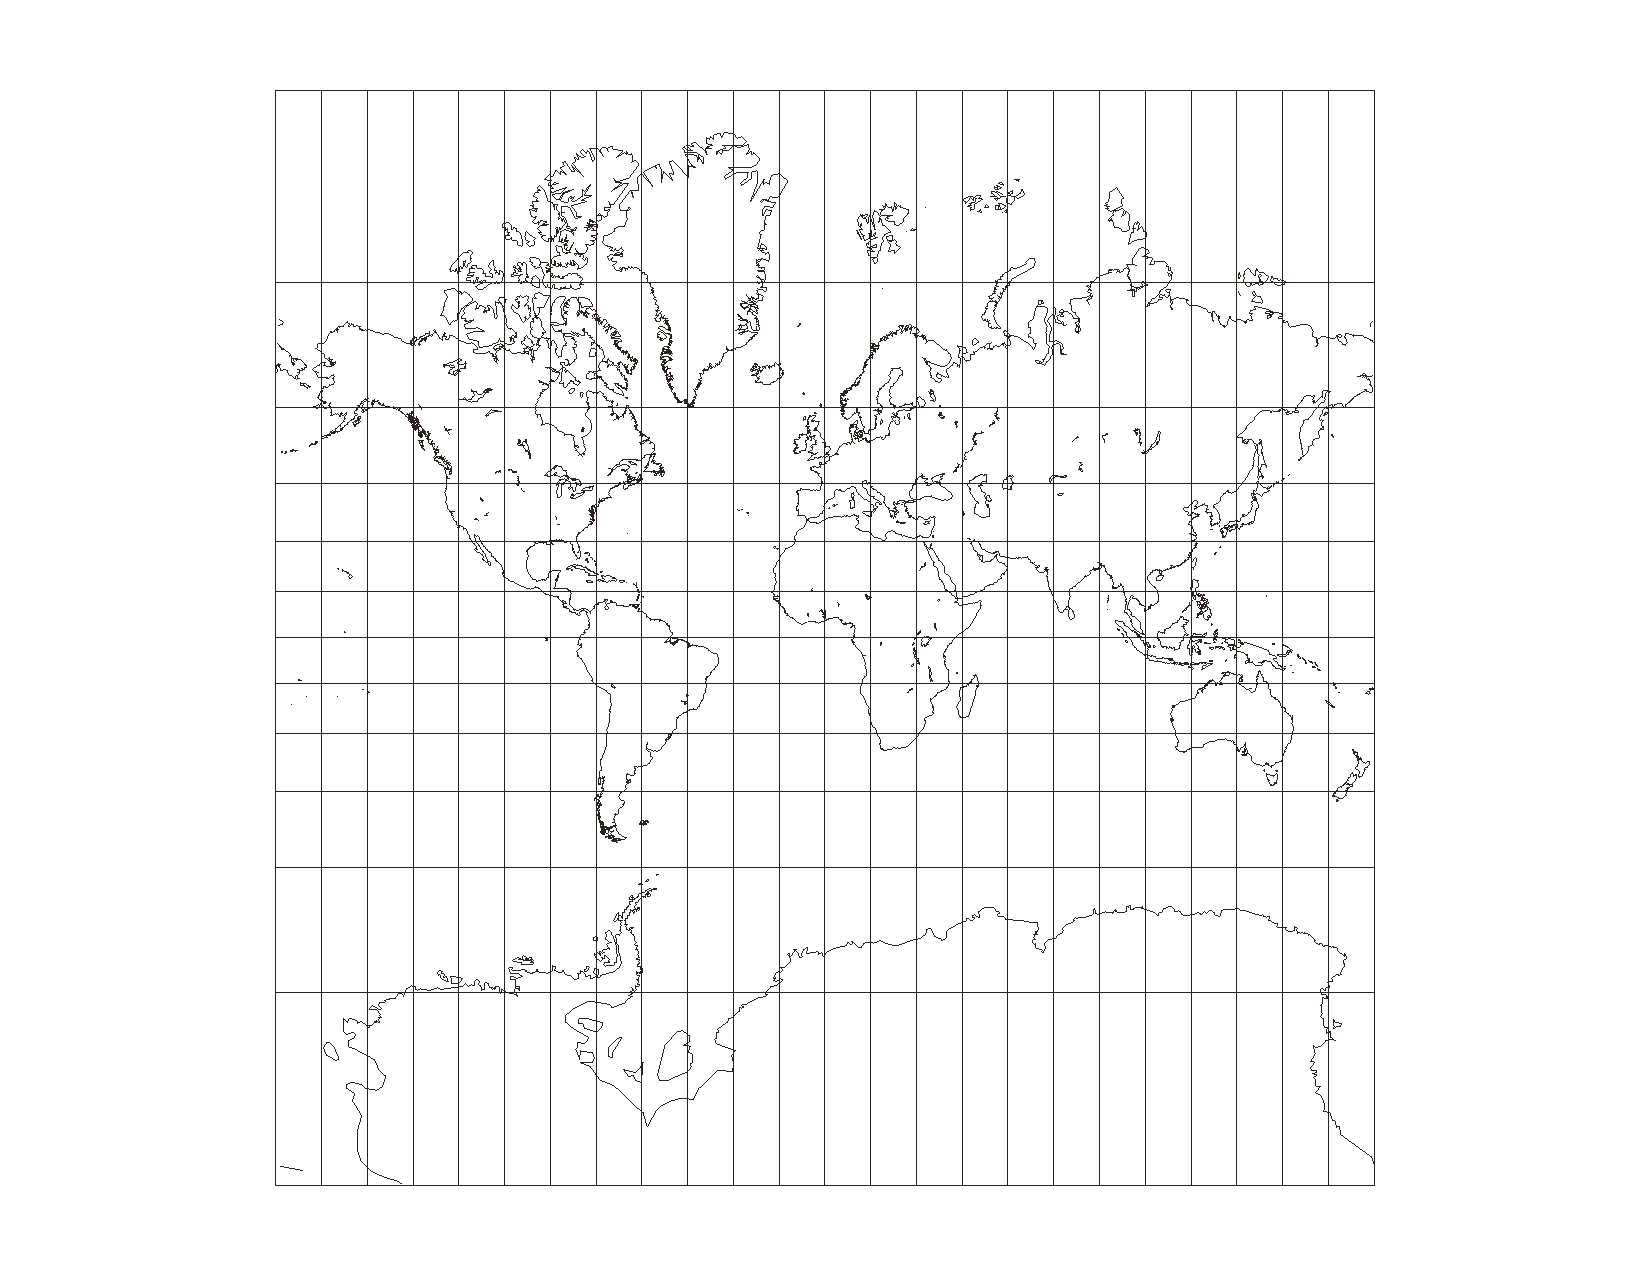
\includegraphics[scale=0.7]{mercator}\\
\caption{Mapamundi en proyección de Mercator.}
\label{fg:mercator}
\end{center}
\end{figure}

La proyección de Mercator, ideada en 1569 por el cartógrafo flamenco Gerhard Kremer,%
\footnote{El nombre «Kremer » significa «mercader». «Mercator » es una versión latinizada de este 
nombre.}
 es la que se utiliza para confeccionar la gran mayoría de las cartas náuticas. Es una 
proyección conforme, en la que los meridianos se representan como líneas verticales, y 
los paralelos como líneas horizontales (figura\ref{fg:mercator}). Todos los demás círculos máximos 
(líneas ortodrómicas) se representan mediante curvas. Por el contrario, las líneas que 
siguen un rumbo constante (loxodrómicas) se representan como líneas rectas. Como 
hemos visto, esta es la propiedad más importante de esta proyección desde el punto de 
vista de la navegación. Sin embargo, la proyección de Mercator tiene el inconveniente de 
que la superficie de los continentes e islas resulta alterada, de tal manera que las 
tierras situadas en latitudes altas aparecen aumentadas con respecto a las situadas cerca del 
Ecuador. Así, Groenlandia aparece en las cartas mercatorianas con un tamaño similar al de 
África, cuando en realidad ésta es mucho mayor. 

%-------------------------------------------------------------------------------
\subsection{Escala de las cartas }

\index{carta!escala|textbf}
\index{escala|textbf}
\index{escala!\textemdash|seealso{carta}}

La escala de una carta es la relación entre el tamaño de los objetos representados en la 
carta y el tamaño real de los mismos en la superficie de la Tierra. Por ejemplo, si la escala 
es $1/100\,000$, una línea de 1~cm en la carta representa una distancia real de 1~km 
($=100\,000\,\mbox{cm}$). Por tanto, cuanto mayor es la escala de una carta, con mayor detalle se 
representará en ella la superficie terrestre.%
\footnote{Puesto que la escala se representa mediante una fracción cuyo numerador es igual a la unidad, 
será tanto mayor cuanto menor sea el valor del denominador. Así, una escala de $1/50\,000$ es 
mayor que una de $1/100\,000$. }

\begin{figure}[hbtp]
\begin{center}
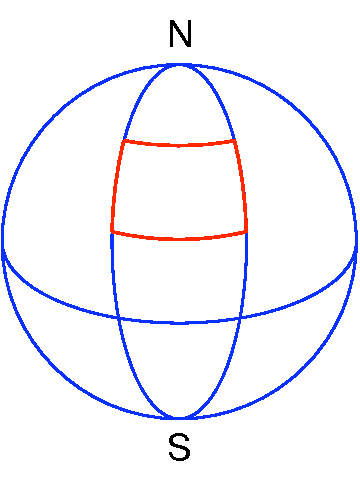
\includegraphics[scale=0.45]{convergencia}\\
\caption{Convergencia de los meridianos.}
\label{fg:convergencia}
\end{center}
\end{figure}

En las cartas mercatorianas  la escala  no es uniforme,  sino que aumenta con la latitud. La razón de ello estriba en la necesidad de que la proyección sea conforme. Mientras que un arco de meridiano de 1'  mide lo mismo en todas las latitudes (1milla náutica),%
\footnote{Salvo una pequeña diferencia debida a la falta de esfericidad de la Tierra.}
un arco de paralelo de 1' sólo sólo mide 1 milla en el Ecuador. A medida que se avanza hacia latitudes más 
altas, los meridianos se van acercando (figura~\ref{fg:convergencia}), por lo que la longitud de los paralelos 
va disminuyendo con la latitud, de tal manera que en la latitud $\phi$ la longitud de un arco de 
1’ de paralelo es igual a $\cos \phi$ millas. Como en la proyección de Mercator la separación entre las líneas rectas que representan los meridianos es constante e independiente de la latitud,  es necesario aumentar la escala en el sentido de la latitud para mantener la proporción entre la medida de los arcos de meridiano y de paralelo en todas las latitudes.
Ésta es la razón por la cual las tierras situadas cerca de los Polos parecen mayores que las que están cerca del Ecuador. 

La figura \ref{fg:escalas-lat-long} muestra la representación en una carta mercatoriana de un rectángulo de 
1’ de latitud por 1’ de longitud. La relación entre la medida en la carta de los lados del rectángulo es $y = x/\cos \phi$,
siendo $\phi$ la latitud del lado inferior. 
Para diferentes latitudes tenemos:
\[ 
\begin{array}{rr}
\multicolumn{1}{c}{\phi} & y \\ \hline
0º & x \\
30º & 1.15 x\\
45º & 1.41 x \\
60º & 2.00 x\\
\end{array}
\]
Por tanto, cuanto mayor sea la latitud tanto mayor será la relación entre el lado vertical y el horizontal del rectángulo. Como la longitud del lado vertical es siempre la misma, 1~milla, vemos que la escala aumenta con la latitud.

\begin{figure}[hbtp]
\begin{center}
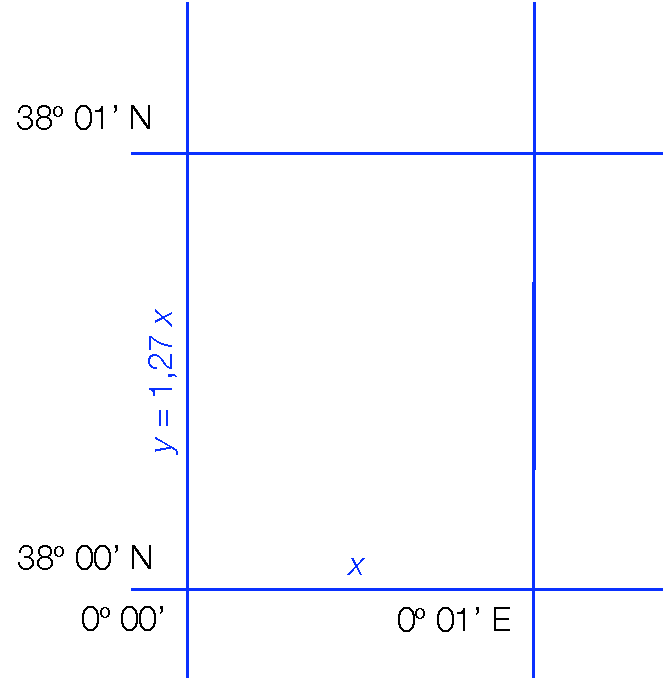
\includegraphics[scale=0.50]{escalas-lat-long}\\
\caption{Escalas de latitud y longitud.}
\label{fg:escalas-lat-long}
\end{center}
\end{figure}

%------------------------------------------------------------
\subsection{Otras proyecciones}

\index{proyección!gnomónica}
\index{proyección!gnomónica polar}
\index{proyección!polar estereográfica}
\index{proyección!de Lambert}
\index{derrota!ortodrómica}

La proyección de Mercator no es adecuada para representar las zonas polares, ya que por 
encima de los 60º de latitud la distorsión introducida por el aumento de la escala es muy 
grande, y los Polos no tienen representación. Por este motivo en las cartas de estas zonas 
se utilizan otras proyecciones, de las que la más común es la \emph{proyección gnomónica}. Ésta 
consiste en proyectar geométricamente la superficie terrestre desde el centro de la Tierra 
sobre un plano tangente a la misma. Cuando el punto de tangencia coincide con uno de los 
polos terrestres se denomina \emph{proyección gnomónica polar}. En este caso los meridianos se 
representan como rectas convergentes en el Polo, y los paralelos como circunferencias 
concéntricas con centro en el Polo. Otras proyecciones de uso frecuente en las cartas de las 
zonas polares son la \emph{proyección polar estereográfica} y la 
\emph{proyección de Lambert modificada}. 

La proyección gnomónica tiene la propiedad de que todos los círculos máximos se 
representan en las cartas como líneas rectas. Por este motivo a veces se usan cartas en pro- 
yección gnomónica oblicua (es decir, con el punto de tangencia en un lugar cualquiera de 
la superficie terrestre) para trazar derrotas ortodrómicas, es decir las que siguen un arco 
de círculo máximo. 

%===================================
\section{Características de las cartas}

\index{cartas náuticas!características}

Las cartas náuticas contienen numerosos detalles interesantes para la navegación, por lo 
que a veces su lectura puede resultar complicada a primera vista. Es necesario, por tanto, 
conocer los convenios de signos, rotulación, escalas, etc. que se utilizan en su confección, 
así como los procedimientos adecuados para mantenerlas al día. A continuación se resumen las características más importantes de las cartas oficiales españolas publicadas por el 
IHM (Instituto Hidrográfico de la Marina), que son similares a las de otros organismos. 
Características generales  

%--------------------------------------------------------------
\subsection{Identificación }

\index{cartas náuticas!identificación}

Las cartas náuticas se identifican mediante un número, que aparece en la esquina inferior 
derecha y en la superior izquierda de cada carta. Cerca del número situado en la esquina 
inferior derecha aparece también el número y la fecha de la edición, y la fecha de la última 
corrección efectuada en el momento de adquirir la carta (figura \ref{fg:id-carta}). 

\begin{figure}[htbp]
\begin{center}
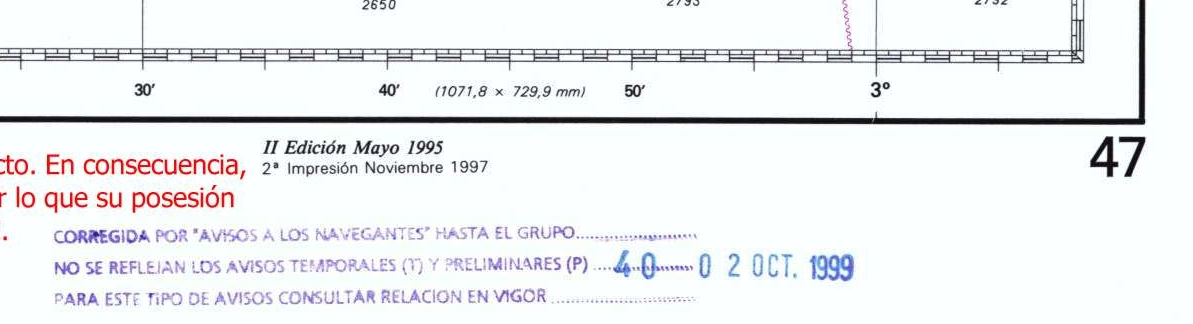
\includegraphics[width=\textwidth]{numero-carta}\\
\caption{Datos de identificación de la carta número 47 del IHM.}
\label{fg:id-carta}
\end{center}
\end{figure}

%--------------------------------------------------------------
\subsection{Tarjeta}
 
\index{cartas náuticas!características}

La mayoría de la información general sobre la carta se encuentra en la \emph{tarjeta}, que es la 
parte de la carta donde se describe la zona que abarca la carta, junto con otros datos de 
interés (figura \ref{fg:tarjeta}). 

\begin{figure}[hbtp]
\begin{center}

\includegraphics[width=\textwidth]{tarjeta}\\
\caption{Tarjeta de la carta número 47 del IHM.}
\label{fg:tarjeta}
\end{center}
\end{figure}

%--------------------------------------------------------------
\subsection{Escala}

\index{carta!escala}
\index{escala}

La escala de la carta es, como hemos visto, la relación entre el tamaño de los objetos 
representados en la carta y su tamaño real sobre la superficie terrestre. Como en la proyección de Mercator la escala varía con la latitud, la escala que figura en la tarjeta se 
refiere siempre a una latitud determinada. Las cartas tienen también escalas gráficas de 
latitudes y longitudes en sus bordes, que permiten leer las coordenadas de un punto cualquiera y medir distancias, tal como se explica más adelante. Por ejemplo, la escala de la 
carta nº 47 del IHM es de 1:350 000 en la latitud 38º 30’ N (figura \ref{fg:tarjeta}). En esta misma 
carta, la escala es ligeramente mayor en latitudes más altas, y ligeramente menor en latitudes más bajas. 

\subsubsection{Escalas de latitudes y longitudes }

\index{carta!escala gráfica}
\index{escala!gráfica}

Las cartas náuticas llevan dos tipos de escalas gráficas, que se utilizan para medir coordenadas y distancias (figura \ref{fg:escala-grafica}): 
\begin{itemize}
\item La \emph{escala de latitudes} está situada en los bordes laterales de la carta. Se usa para 
medir la latitud de un punto en la carta. También se usa para medir distancias, ya 
que 1~M = 1’ de latitud. 
\item \emph{La escala de longitudes} está situada en los bordes superior e inferior. Se usa para 
medir longitudes sobre la carta. 
\end{itemize}

\begin{figure}[hbtp]
\begin{center}
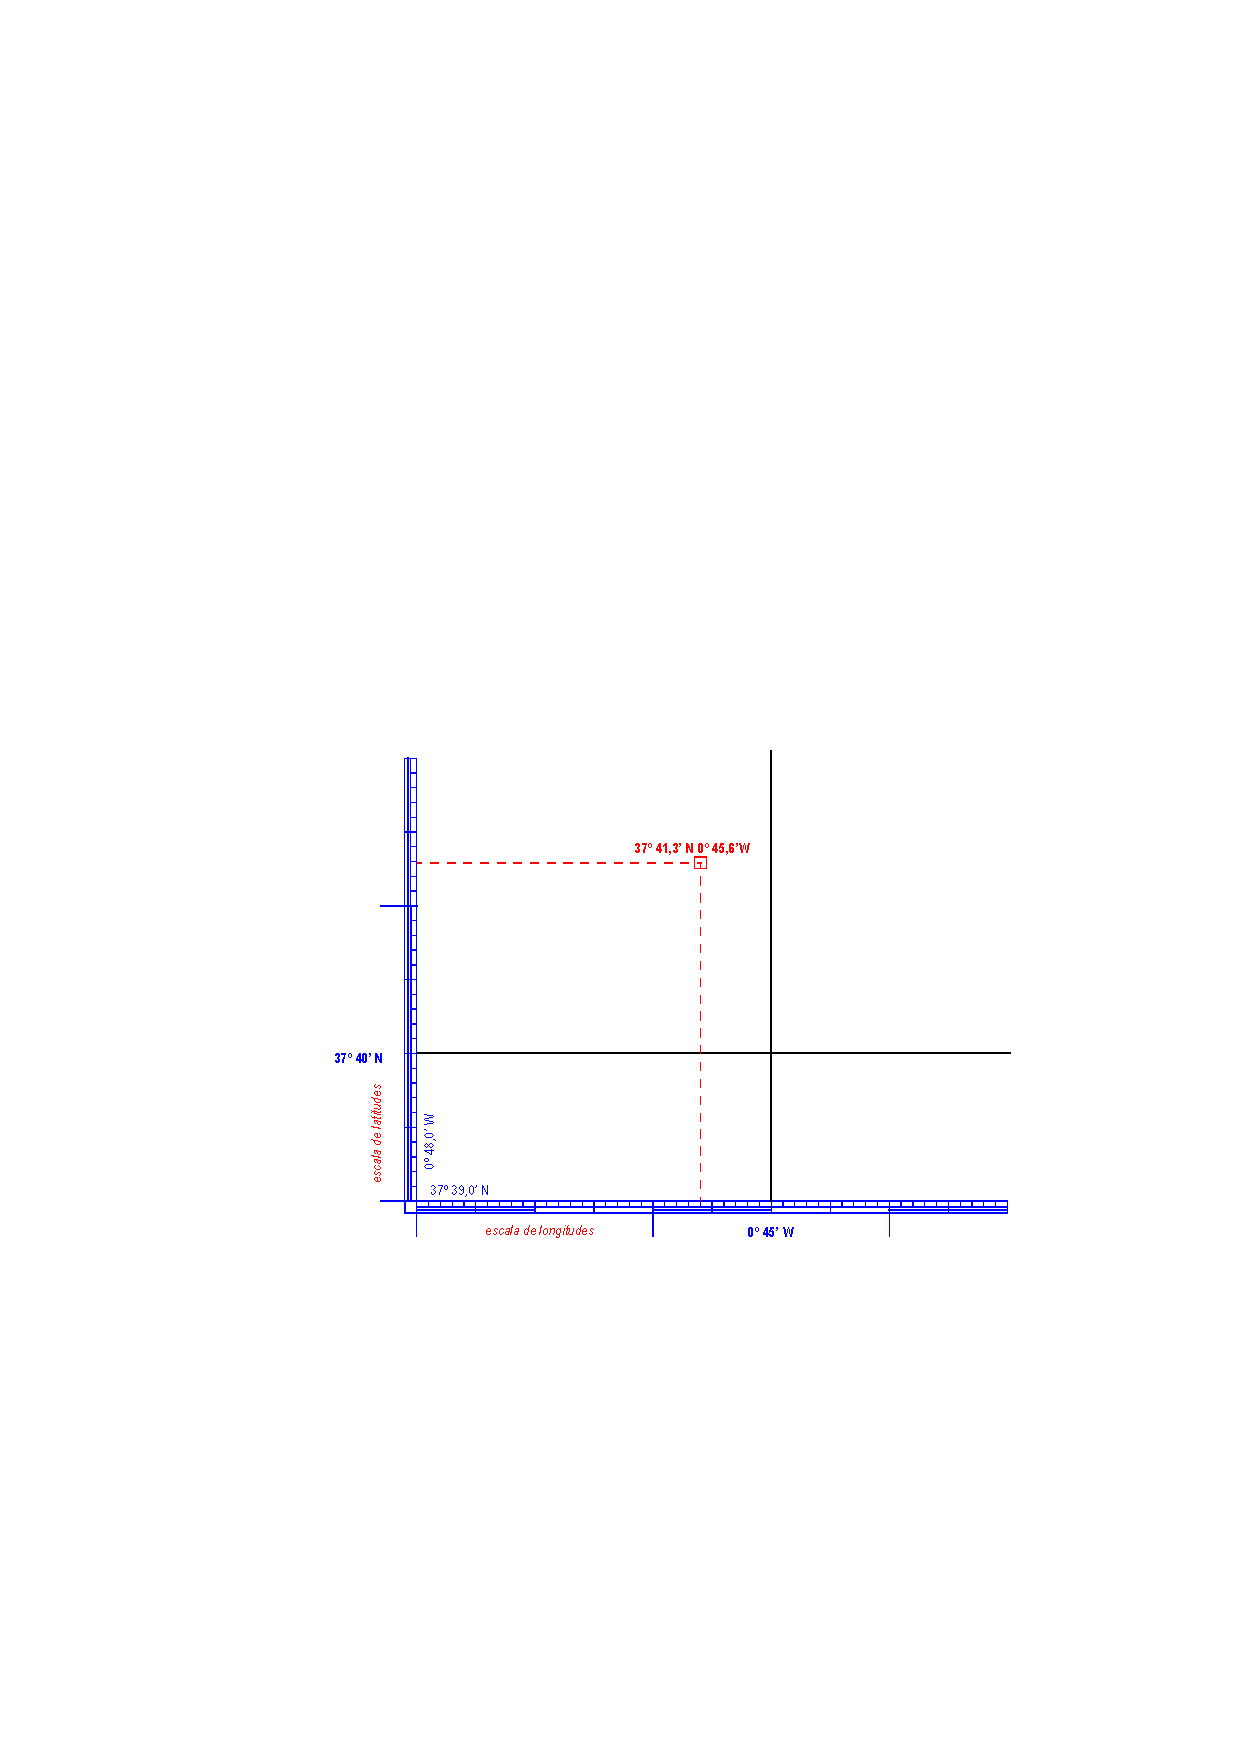
\includegraphics[width=\textwidth]{escala-grafica}\\
\caption{Escalas de latitud y longitud.}
\label{fg:escala-grafica}
\end{center}
\end{figure}

\begin{ejemplo}
El punto marcado en la carta de la figura  \ref{fg:escala-grafica} está situado en 37º 41,3’ N  0º 45,6’ W.
\end{ejemplo}

%--------------------------------------------------------------
\subsection{Tipos de cartas}

\index{cartas náuticas!tipos}
\index{cartas!generales}
\index{cartas!de arrumbamiento|seealso{cartas de recalada}}
\index{cartas!de recalada}
\index{cartas!de navegación costera}
\index{aproche}
\index{portulano}
\index{carta!cartucho}

Las cartas se clasifican según su escala y la superficie de la Tierra que representan en: 
\begin{itemize}
\item \emph{Cartas generales}: las que representan una gran extensión de la superficie de la 
Tierra, con escalas comprendidas entre 1:30\,000\,000 y 1:3\,000\,000.Se utilizan 
únicamente para trazar grandes derrotas en navegación oceánica. 
\item \emph{Cartas de arrumbamiento} o \emph{recalada}: representan una extensión limitada de la 
superficie terrestre, con una escala comprendida entre 1:3\,000\,000 y 1:200\,000. 
Se utilizan para navegar en distancias medias o para acercarse a la costa después 
de una navegación de altura. 
\item \emph{Cartas para navegación costera}: representan de forma detallada una porción de 
costa, con una escala comprendida entre 1:200\,000 y 1: 50\,000. 
\item \emph{Aproches}: son cartas de gran escala (del orden de 1:25\,000), que se utilizan para 
navegar cerca de los puertos o en zonas de gran dificultad. 
\item  \emph{Portulanos}: con escala mayor de 1:25\,000. Representan con gran detalle el interior 
de los puertos, canales y fondeaderos. 
\end{itemize}
Los aproches y portulanos se encuentran a menudo insertados en forma de 
\emph{cartucho} en otras cartas de menor escala. 

\index{cartas!de punto menor}
\index{cartas!de punto mayor}

También se habla de cartas de \emph{punto menor} o de \emph{punto mayor}. Se consideran cartas de 
punto menor las cartas generales y las de arrumbamiento, y cartas de punto mayor las restantes. 

%--------------------------------------------------------------
\subsection{Datum de la carta} 

\index{datum}
\index{datum!horizontal}

\index{datum!europeo (Potsdam)}
%\index{sistema geodésico mundial|see{WGS84}}
%\index{World Geodetic System|see{WGS84}}
\index{coordenadas!geográficas}
 
La tarjeta también contiene información sobre el \emph{datum horizontal} de la carta. Como 
vimos en el capítulo \ref{ch:introduccion}, este término se refiere al sistema de referencia que 
que se utiliza para determinar las coordenadas geográficas sobre la superficie de la Tierra. 
Actualmente las cartas españolas se refieren al \emph{sistema geodésico mundial} (WGS\,84), 
que es el que se utiliza en la mayoría de los países y 
en los sistemas de navegación por satélite  (ver capítulo \ref{ch:satelite}). Sin embargo, todavía se encuentran cartas referidas al  \emph{datum europeo de 1950}. Con el fin de permitir el uso de estas cartas en la navegación por satélite, la tarjeta proporciona instrucciones para convertir las coordenadas geográficas medidas en la carta al sistema WGS84 y 
viceversa. 

%\begin{figure}[hbtp]
%\begin{center}
%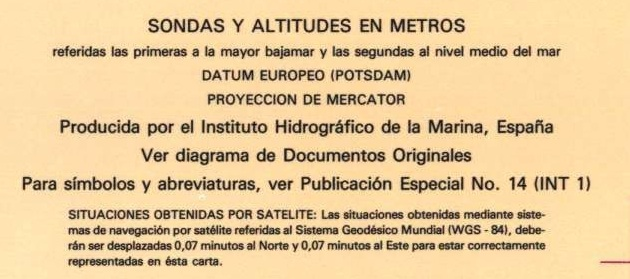
\includegraphics[width=\textwidth]{datum-europeo}\\
%\caption{Tarjeta de una carta referida al datum europeo.}
%\label{fg:datum-europeo}
%\end{center}
%\end{figure}

\begin{ejemplo}
En la tarjeta de de una carta referida al datum europeo %(figura\ref{fg:datum-europeo})
figura el siguiente párrafo: 
\begin{quotation}\noindent\itshape
SITUACIONES OBTENIDAS POR SATÉLITE: Las situaciones obtenidas mediante sistemas 
de navegación por satélite referidas al Sistema Geodésico Mundial (WGS-84) deberán ser 
desplazadas 0,07 minutos al Norte y 0,07 minutos al Este para estar correctamente representadas en esta carta. 
\end{quotation}
Si se ha obtenido una situación por satélite referida al sistema WGS84 igual a 37º44,02’\,N
0º42,35’\,W, la trazaremos en la carta como 37º44,09’\,N 0º42,28’\,W. En una carta de punto mayor
la diferencia es imperceptible (0,4\,mm, aproximadamente, para una escala de 1:300\,000), pero si usamos cartas de 
punto mayor es muy importante hacer la correción del datum. Así, por ejemplo, la corrección de 0,07’ 
de latitud (129,6\,m) equivale a 2,6\,mm en una carta de escala 1:50\,000, y a 8,6\,mm en un portulano de escala
 1:15\,000.
\end{ejemplo}

Como vemos en el ejemplo anterior, cuando se quiere obtener situaciones precisas con 
sistemas de navegación por satélite es necesario tener en cuenta el datum de la carta y 
hacer las correcciones necesarias. 

\subsubsection{Datum vertical }

\index{datum!vertical}
\index{bajamar escorada}

El \emph{datum vertical} es la referencia que se usa para medir las elevaciones (en tierra) y las 
sondas (en la mar). En las cartas españolas las elevaciones se miden siempre en metros 
sobre el nivel medio del mar, y las sondas también en metros, referidas a la bajamar 
escorada (ver capítulo \ref{ch:mareas}). 

En las cartas inglesas y norteamericanas antiguas se miden las elevaciones en pies (ft),%
%\footnote{\emph{Feet}.} 
 y las sondas en brazas (fm)%
%\footnote{\emph{Fathoms}.}
 y pies, aunque en las cartas modernas estas magnitudes se 
miden en metros. En estas cartas las sondas se refieren al nivel medio de la bajamar de 
mareas vivas. 

%--------------------------------------------------------------
\subsection{Rosa náutica y declinación magnética}

\index{rosa}
\index{rosa!náutica}
\index{rosa!de los vientos|see rosa náutica}
\index{declinación!magnética}
\index{declinación!variación anual}

Una rosa náutica es una figura consistente en dos círculos graduados concéntricos que indican 
rumbos verdaderos y magnéticos, respectivamente (figura \ref{fg:rosa}). 
En la dirección que señala el Norte magnético se indica el valor de la declinación magnética 
para un año determinado, y el valor de la variación anual de la misma. 
Cuando la declinación magnética varía significativamente de una parte a otra de la 
carta, su valor se indica mediante distintas rosas o con rótulos adicionales. En estos casos 
hay que emplear el valor de la declinación indicado en la rosa o rótulo más próximo a la 
zona de la carta con la que se esté trabajando. 

\begin{figure}[htbp]
\begin{center}
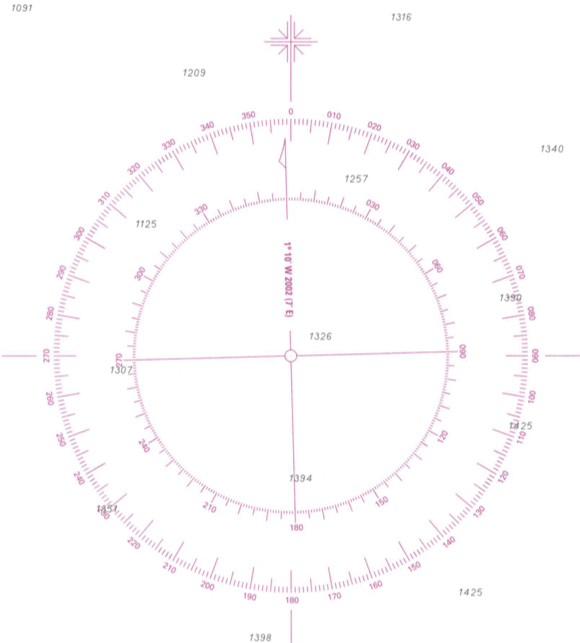
\includegraphics[scale=0.5]{rosa}\\
\caption{Rosa náutica.}
\label{fg:rosa}
\end{center}
\end{figure}

\begin{ejemplo}
El valor de la declinación magnética en la zona de la carta donde se encuentra la rosa 
de la figura \ref{fg:rosa} es de 1º10’\,W en 2002. La variación anual es de 7’\,E. 
Por tanto, en 2009 la declinación será:
\[
\begin{array}{lcll}
  \mbox{Valor en 2002} & =  & -1º \, 10' \: \mathrm{(W)} \\
  \mbox{Variación}     & =  & +0º \, 42' \: \mathrm{(E)} & (\mbox{7 años} \times 10' )\\
%  \cline{3-5}\\
\mbox{Valor en 2009}  &  = &   -0º \, 25’ \: \mathrm{(W)} & \approx -0,5º 
\end{array}
\]
El valor de la declinación en 2003, por tanto, es aproximadamente $-0,5º$. 
\end{ejemplo}

%%%%%%%%%%%%%%%%%%%%%%%%

\subsubsection{Detalles de las cartas}

Las figuras 2.9 y 2.10 muestran sendos fragmentos de dos cartas náuticas: el aproche a la 
ría de Cedeira incluido en la carta nº930, y la carta de navegación costera nº471A del 
IHM. En ambas se pueden apreciar la mayoría de los detalles que suelen aparecer en las 
cartas náuticas. 

Signos y abreviaturas 

La publicación especial nº 14 (INT 1) del Instituto Hidrográfico de la Marina contiene 
todos los símbolos, abreviaturas y términos usados en las cartas oficiales españolas. Los 
símbolos son los recomendados por la Organización Hidrográfica Internacional (OHI), 
aunque en algunos casos las cartas españolas de una cierta antigüedad utilizan símbolos 
nacionales distintos de aquéllos. Estos símbolos nacionales se explican también en la 
publicación nº 14. 


Profundidad y naturaleza del fondo 
La profundidad medida en distintos puntos 
de la carta se indica mediante sondas. Las 
sondas se refieren al datum vertical de la 
carta (la bajamar escorada en las cartas espa- 
ñolas), y se representan mediante números 
que indican la profundidad en metros y, en su 
caso, en decímetros, en el punto donde se 
encuentran. La cifra que indica los decíme- 
tros se escribe como un subíndice de las que 
indican los metros enteros. Las sondas que se 
encuentran fuera de posición, es decir las que 
se refieren a un punto cercano a aquél donde 
se encuentran, se escriben entre paréntesis. 
La sondas medidas con precisión se escriben 
en cursiva, mientras que las dudosas o las 
obtenidas de otros documentos menos fiables 
se escriben con cifras rectas (figura 2.8). 
Las sondas negativas corresponden a 
puntos que velan en la bajamar escorada, aunque pueden quedar sumergidos al subir la 
marea (capítulo 8). Se escriben subrayadas. 

Ejemplo 2.5. En un punto en donde la carta marca 18 la profundidad del agua es igual a 0,7m cuando 
la altura de la marea es de 2,5m. Cuando la altura de la marea es menor de 1,8m el punto vela (es 
decir, está fuera del agua). 


Las sondas suelen ir acompañadas de una
abreviatura, situada debajo de ellas, que
indica la naturaleza del fondo. La figura 2.11
muestra algunas de las abreviaturas más
comunes definidas por las normas nacionales
e internacionales. 
Los veriles o líneas isobáticas son líneas
que unen todos los puntos que tienen una
misma profundidad (por ejemplo, 10m, 20m
o 100m). Las zonas delimitadas por los veri-
les de menor profundidad, dependiendo de la
escala y del tipo de carta, se colorean con dis-
tintos tonos de azul. La zona cercana a la
costa que queda al descubierto en la bajamar
se colorea de verde claro. 
 Peligros 
Los distintos peligros que se encuentran en la
mar, como piedras, bajos, restos de naufra-
gios, etc. se indican en las cartas mediante
diversos signos, los más importantes de los
cuales se muestran en la figura 2.12. 
Marcas y luces 
Las cartas muestran de forma detallada la
situación de las marcas terrestres útiles para la
navegación, y de las boyas, balizas, luces y
otras ayudas. Las luces se indican con una
marca púrpura, junto con sus características
luminosas (figura 2.13). Los sectores visibles
o de distintos colores, en su caso, se indican
también gráficamente en la carta. También se
indica la altura de la luz sobre el nivel medio
del mar y su alcance en millas. Todos estos
datos se encuentran igualmente en el Libro de 
Faros, donde debe acudirse siempre para una 
referencia más completa y exacta. 
V, G Verde (green). 
Figura 2.13. Símbolos y abreviaturas 
de luces y faros.

Puesta al día de las cartas 
La información que contienen las cartas sólo es exacta en la fecha de su última actualiza- 
ción, que en el momento de su adquisición está escrita en el margen inferior (figura 2.4). 
Para mantenerlas al día es preciso actualizarlas con las correcciones que se publican cada 
semana en los Avisos a los navegantes, editados por el Instituto Hidrográfico de la 
Marina. 

%===================================
\section{Trabajo sobre la carta}


%===================================
\section{Cartas electrónicas}


\appendix
%-------------------------------------------------------------
% $Id$
% © Juan A. de la Puente, 2008
%-------------------------------------------------------------
\chapter{Rumbos cuadrantales y por cuartas}
\label{ch:rumbos}
%===================================
%-------------------------------------------------------------
\backmatter
\chapterstyle{default}
% glosario
%\include{glosario}
%\bibliographystyle{}
%\bibliography{biblio}
%\nocite{*}

%\clearpage
%\pagestyle{index}
\indexintoc
\printindex

%In older books it was often the custom to have a colophon as the final element in a book. 
%This is an inscription which includes information about the production and design of the 
%book and nearly always indicates which fonts were used.

%% colofón 
%El colofón es el último párrafo que se encuentra en el texto de la obra, en él se halla el lugar de impresión, nombre del impresor y fecha.
%-------------------------------------------------------------
% $Id$
% © Juan A. de la Puente, 2008
%-------------------------------------------------------------
% Colofón
%-------------------------------------------------------------
\cleardoublepage
\pagestyle{empty}
\null\vfil

\begin{adjustwidth}{3cm}{3 cm}
\begin{center}
{\Large\textsf{Colofón}}
\end{center}
\begin{center}
Compuesto con \LaTeX y la clase \textsf{memoir}.  

%This manual was typeset using the LaTeX typesetting system
%created by Leslie Lamport and the memoir class. 
%The body text is set 10/12pt on a
%33pc measure with Computer
%Modern Roman designed by Donald Knuth. Other fonts include
%Sans, Smallcaps, Italic, Slanted and Typewriter, all from Knuth's 
%Computer Modern family.

\end{center}

\end{adjustwidth}

\vfil



\end{document}